\documentclass[letterpaper,11pt]{article}
\usepackage{hyperref}
\usepackage{wrapfig}
\usepackage{tikz}
\newcommand{\superscript}[1]{\ensuremath{^{\textrm{#1}}}}
\newcommand{\unit}[1]{\ensuremath{\, \mathrm{#1}}}

\begin{document}

\title{Machine Learning Independent Study Project\\ Analysis of CS 415 Students}
\date{January 12, 2012}
\author{Carmen St.\ Jean}

\maketitle

\section{Background}

At the University of New Hampshire, many freshmen enroll in CS 415 (Introduction to Computer Science I), but only a few graduate with a B.S. in computer science years later.  This has left the Computer Science Department wondering why the retention rate is so low and what could be done to address this issue.  As both a former CS 415 student and more lately a teaching assistant for the course, I have wondered how correlated a student's performance in CS 415 is to how well that student does in the major as a whole.

Success in an introductory level course would usually be followed by a like-wise successful academic career, but not always.  In CS 415, there are many opportunities where students are encouraged to work together and help each other - behaviors which are discouraged or considered plagiarism in higher-level courses.  Furthermore, students can also attend the Programming Assistance Center (PAC) regularly for help or ask for personal tutors, but this help is not available after the first year.  Given these factors, it is possible for students to earn a decent grade in CS 415 but struggle in later courses and even leave the major.

The CS 415 course is constantly evaluating students' performances with one programming assignment, one recitation assignment, one quiz, and two lab assignments every week, plus three on-line exams and three on-line written exams throughout the semester.  One of these aspects of a student's grade may be more telling than others, such as the quiz average since that is one of the few times students cannot ask for help.  Additionally, other factors such as class standing, declared major, or sex could also be significant.

\section{Problem}
%\section{What is being investigated?}

I visited Mark Bochert, Dan Bergeron, Phil Hatcher, and Radim Bartos to discuss investigating CS 415 student grades and we came up with the following questions to investigate:

\begin{itemize}
\item Does a student's performance in CS 415 indicate much about overall success in the major?

[Will we see that there are A students who fail subsequent courses (or disappear for other reasons such as changing majors)?  Are there students who get a C that graduate within the major later?]
\item Do particular characteristics of a CS 415 student's or aspects of the student's grade indicate seem to heavily influence the student's overall success?

[Does the quiz average say the most about a student's abilities?  Is there a homework assignment that is more meaningful than others?  The first assignment?  The last assignment?]
\item Concerning the overall CS 415 grade, is there a threshold that students must cross in order to pass later courses such as CS 416, CS 515, and CS 520?

[Does a student need to get at least a B in order to not fail CS 520 a few years later?]
\end{itemize}

\section{Justification}

We all realized that pessimistic conclusions could be drawn from the data, particularly if we find that students must do extremely well in CS 415 in order to have a good chance of graduating with a computer science degree.  One could say that such results could be used to design interventions with students who, according to the model, seem unlikely to finish the major, though basing advising decisions solely on the results of a project would not be appropriate.

I entered this study hoping to draw more positive conclusions from the study.  As a teaching assistant for CS 415, I am often approached by discouraged students who are considering changing majors.  Many of them seem both determined and capable, but their grades may not accurately reflect that.  Sometimes they are even further disheartened after comparing themselves to other students, when the other students might have deceptively high grades from heavily seeking help.

My hope was for this project to find that there are students who do not perform perfectly in CS 415 but finish the major without a significant struggle.  That might be encouraging news for the more worried students whose biggest problem is self confidence.  Yet, it would again be inappropriate to base advising decisions on a mere project, even if it is to encourage someone to stay in the major despite falling grades.

More concretely, the Computer Science Department may find other ways to apply the results of this study.  It could be a step closer to understanding why some students ultimately leave the major.  Or, more discretely, it could help to establish minimum grade requirements or to see if restructuring of CS 415 is necessary.

\section{Why machine learning?}

This is a machine learning problem because we can apply linear regression to the numerical questions (i.e., grade predictions) and logistic regression to the categorical questions (i.e., whether or not students will enroll in other courses or finish the major).

In machine learning, linear regression is an approach to modelling the relationship between an output and one or more explanatory variables.  It can be used to create a predictive model and also to determine the strength of the relationship between each explanatory variable and the output or if no relationship exists at all.  Linear regression can be used to determine which variables matter to a student's overall success and, given the grades of a more recent group of students, attempt to predict future grades.

Logistic regression is another machine learning technique that operates like linear regression, but is used for determining the probability of a binary outcome.  E.g., this will be used to determine how likely a student is to graduate within the major.  Linear regression should not be used for problems with binary dependent variables because it can produce predictions that are not on a 0 to 1 scale.  Logistic regression can keep predictions on a 0 to 1 scale by transforming the probabilities to odds and taking the natural logarithm of these odds.

\section{Strategy}

The above questions were explored for students enrolled in CS 415 during the following semesters:

\begin{itemize}
\item Fall 2007
\item Fall 2008
\item Fall 2009
\item Fall 2010
\end{itemize}

Mark Bochert, Phil Hatcher, and Carolyn Kirkpatrick provided anonymized data about students from the above semesters that to make up all of the features and outputs for the machine learning problems.

The features of our logistic and linear regression models were made up of the students' grades as well as sex, declared major while in CS 415, class standing while in CS 415, and which mathematics the students were enrolled in (if any) while taking CS 415.  The outputs investigated were:

%\begin{itemize}
%\item CS 415 grades
%    \begin{itemize}
%    \item Homework programs
%    \item Preliminary homework assignments
%    \item Labs
%    \item Recitations
%    \item Quizzes
%    \item On-line exams
%    \item Written exams
%    \item Final grade
%    \end{itemize}
%\item Sex
%\item Declared major while in CS 415
%\item Class standing while in CS 415
%\item Which mathematics course (if any) the student was enrolled in while in CS 415
%\end{itemize}

%The outputs that were investigated were:

\begin{itemize}
\item Whether the student will take CS 416
\item CS 416 grade (if the student took 416)
\item Whether the student will take CS 515
\item CS 515 grade (if the student took 515)
\item Whether the student will take CS 520
\item CS 520 grade (if the student took 520)
\item If the student graduated with a CS degree (for fall 2007 and fall 2008 students declared as CS majors only)
\end{itemize}

Both the features and outputs are explained in detail in further sections.

For the outputs that involved YES/NO answers, logistic regression was used, while linear regression was used for the outputs involving continuous values.

The Weka machine learning software suite\cite{weka:weka} was used to perform these regressions on the data.  All linear and logistic regression was performed using leave-one-out cross-validation. Additionally, Microsoft Excel and Weka were used for preprocessing of the features.

\section{Features}

Features in machine learning problems are also known as explanatory variables, denoted by X.  The features available to our model were a combination of numerical and categorical features, totalling 56 features in all.

\subsection{Numerical Features}

The grade values, being continuous data, were represented as numerical features in our model.

\subsubsection{Description of Raw Numerical Features}

Mark Bochert provided the following grade information for 346 students from the fall semesters of 2007, 2008, 2009, and 2010:

    \begin{itemize}
    \item Homework programs - Students individually complete a program approximately once a week, for a total of about twelve per semester.  They are allowed to visit the Programming Assistance Center to receive help and may talk with fellow students about the assignment on a conceptual level.
    \item Preliminary homework assignments - Some early assignments require students to prepare something such as a UML diagram in advance.  There are about five of these assignments per semester.
    \item Labs - Twice a week, students attend a lab where they must complete an assignment.  They are allowed to work with each other and ask for assistance from the teaching assistant or instructor in charge of the lab.
    \item Recitations - Once a week, students attend a recitation where a worksheet is distributed.  They are allowed to work with each other to do this worksheet.
    \item Quizzes - Students take a written quiz once a week that lasts approximately twenty minutes.  The quiz is closed notebook, but they are allowed to prepare a handwritten index card with information on it.
    \item On-line exams - Two or three times a semester, students take an on-line exam during what is normally a lab time.  They must complete four or five programming problems with no assistance from the lab instructor or teaching assistant.  They are allowed to use old assignments and the Internet, but cannot communicate with other students.
    \item Written exams - These exams are usually paired with the on-line exams.  They are closed notebook, but students may bring in an 8.5 by 11 inch sheet of paper with handwritten information.
    \item Final grade - The final grade the student received out of 100.
    \end{itemize}

\subsubsection{Preprocessing of Numerical Features in Excel}

Ideally, every single assignment of all the various types - quizzes, recitations, homeworks, etc - would each be its own feature in our logistic and linear regression models.  This would have allowed us to determine if particular assignments are more significant than others.  However, the assignments varied enough that a lot of preprocessing was required, despite the course having been taught by the same instructor each time.

First, all of the grades had to be normalized to be percentages.  Point values of assignments varied both within and between semesters - e.g., the first written exam of 2009 was out of 42 points and the second was out of 92 points - so each grade received had to be divided by the maximum possible score.  The only exception was homework programs which were always graded out of 100 points.

Second, the actual number of assignments varied across semesters - e.g., 2007 featured only 14 lab assignments, while the other semesters had around 25 labs.  For written exams and on-line exams, where there were either one or two of each per semester, this issue was dealt with by using minimum grade, maximum grade, and average grade as features.  For the other types of assignments, more features were introduced:

\begin{itemize}
\item Average - The average of all assignments of that type.
\item Minimum - The minimum of all assignments of that type.
\item Maximum - The maximum of all assignments of that type.
\item Percentage below 70\% - The percentage of assignments that received a score below 70\%.
\item Percentage Zeros - The percentage of assignments that received a zero.
\item Difference - The average of the first half of the assignments of that type minus the average of the second half of the assignments (e.g., the average of assignments 1-5 minus the average of assignments 6-10).
\end{itemize}

These six features were produced for each of the five remaining assignment types - quizzes, labs, recitations, homework programs, and preliminary assignments - resulting in thirty features.

Finally, the final CS 415 grade, as calculated by the instructor, was also included as a feature.  With the thirty features mentioned above, three features for on-line exams, and three features for written exams, a total of 37 features were produced based on CS 415 grades.

\subsubsection{Preprocessing of Numerical Features in Weka}

All of the features were normalized to a scale from zero to one.  This was done to allow us to compare the absolute values the weights later, which is only possible if all of the weights are on the same scale.

\subsection{Categorical Features}

Categorical features in machine learning problems are used when the data can take on a limited number of possible values.  In our model, categorical variables were used for standing, major, sex, and math class.

\subsubsection{Description of Raw Categorical Features}

Data were gathered about each student enrolled in CS 415 during the 2007, 2008, 2009, and 2010 fall semesters by Mark Bochert, Carolyn Kirkpatrick, and Phil Hatcher:

\begin{itemize}
\item Academic standing while in CS 415:
	\begin{itemize}
	\item Freshman
	\item Sophomore
	\item Junior
	\item Senior
	\item Graduate student
	\end{itemize}
\item Sex:
	\begin{itemize}
	\item Male
	\item Female
	\item Unknown (for some students this information was unavailable)
	\end{itemize}
\item Math course while enrolled in CS 415:
	\begin{itemize}
	\item MATH 302 (Elementary Math II)
	\item MATH 418 (Analysis and Applications of Functions)
	\item MATH 425 (Calculus I)
	\item MATH 426 (Calculus II)
	\item MATH 531 (Mathematical Proof)
	\item None
	\item Unknown
	\end{itemize}
\item Is a Computer Science (CS) major:
	\begin{itemize}
	\item Yes
	\item No
	\end{itemize}
\item Is either an Electrical Engineering or Computer Engineering (ECE) major:
	\begin{itemize}
	\item Yes
	\item No
	\end{itemize}
\end{itemize}

\subsubsection{Preprocessing of Categorical Features in Weka}

Within the Weka program, these were all represented with 1-in-k encoding - i.e., binary features of which only one is marked as true.  Therefore, rather than being five nominal features, there were 19 total binary features, one for each option of each categorical feature.

\section{Outputs}

Outputs in machine learning problems, denoted by y, are also known as dependent variables.  All of the output feature information was provided by Carolyn Kirkpatrick from the Computer Science Department's student records and class rosters.

\subsection{Numerical Outputs}

The letter grades for the following courses were provided for each of the 346 student samples, but only if the students took the courses:

\begin{itemize}
\item CS 416 (Introduction to Computer Science II) - 157 students.
\item CS 515 (Data Structures) - 119 students.
\item CS 520 (Assembly Language Programming and Machine Organization) - 67 students.
\end{itemize}

If the student had multiple grades for a single course after retaking that course, then only the first grade received was considered.  Grades were converted to the official University of New Hampshire numerical grading scale (see Table \ref{table:unhscale}).

\subsection{Categorical Outputs}

The first three of the following categorical features were created based on whether or not a grade was available for the course in question.  The fourth and final categorical feature was created based on information gathered by Carolyn Kirkpatrick.  

\begin{itemize}
\item Took CS 416 after CS 415 (analysed for all 346 students):
	\begin{itemize}
	\item Yes (157 students)
	\item No (189 students)
	\end{itemize}
\item Took CS 515 after CS 416 (analysed for 157 students total):
	\begin{itemize}
	\item Yes (119 students)
	\item No (38 students)
	\end{itemize}
\item Took CS 520 after CS 515 (analysed for 119 students total):
	\begin{itemize}
	\item Yes (67 students)
	\item No (52 students)
	\end{itemize}
\item Took 415 in fall 2007 or fall 2008 while declared a CS major and graduated with a degree in CS (analysed for 70 students total):
	\begin{itemize}
	\item Yes (16 students)
	\item No (54 students)
	\end{itemize}
\end{itemize}

Only the semesters of fall 2007 and fall 2008 were studied for whether or not CS major had successfully managed to graduate with a B.S. in Computer Science because the students from the other two semesters were only juniors or seniors at the time of this study.

\section{Results}

\subsection{Linear Regression Results}


\subsubsection{Measure of Performance}

For comparison, we ran our models on a decision stump rule in addition to linear regression.  Decision stump in Weka does regression based on mean-squared error to make a decision tree from a single feature.  ``CS 416 Grade," ``CS 515 Grade," and ``CS 520" all ended up using the CS 415 final grade feature for the decision stump model.   Table \ref{table:linperform} shows the performances of linear regression against decision stump.

Root relative squared error (RRSE) is a calculation of root mean squared error by the root mean squared error that was obtained by predicting only the mean of the target values.  Thus, an RRSE greater than 100\% means that the model is doing worse than predicting just the mean all of the time.  Judging by the RRSE values in table \ref{table:linperform}, we would be better off error-wise predicting the mean of the CS 520 grades rather than using either linear regression or decision stump.  The other outputs and models performed better but all have relatively high error values in general.

The correlation coefficient is a measure of strength of linear dependence between two variables X (our features) and y (our output), between -1 and 1 (inclusive).  A correlation coefficient of zero means the two variables are completely independent, so the further from zero the better.  The results from Weka in table \ref{table:linperform} showed for ``CS 416 Grade" and ``CS 515 Grade" that linear regression was slightly less correlated than decision stump.  For ``CS 520 Grade", both linear regression and decision stump had almost entirely no correlation.

The small correlation coefficients of ``CS 520" could mean that CS 415 grades are completely unrelated to CS 520 grades, but - given the high error values - it is also possible that there were not enough samples (67) compared to our number of features (56), meaning no conclusion can be drawn.  Perhaps this question could be revisited in the future with more samples to see what results occur.

\subsubsection{Heatmaps}

Heatmaps were produced depicting the frequency of actual versus predicted values for linear regression where the x-axis indicates the actual grade received in the courses and the y-axis indicates the predicted grade received in the courses.  The color in each box represents the number of occurrences for that combination of actual value and predicted value.   An ideal heatmap would contain blue in all of the other squares but the diagonal running from the bottom left to the top right.  This would mean that the predictions were 100\% accurate. 

The heatmaps of the linear regression models - figures \ref{figure:heatmaps1}, \ref{figure:heatmaps3}, and \ref{figure:heatmaps5} -  seem visually closer to the ideal heatmap described above than that of the decision stump models - figures \ref{figure:heatmaps2}, \ref{figure:heatmaps4}, and \ref{figure:heatmaps6}.  Still, even the linear regression models are far from perfect and show a lot of error outside of the diagonal.  The desired diagonal is least discernible in the ``CS 520 Grade" heatmap, which makes sense for two reasons: there were less samples available for this model and this model is attempting to predict further into the future than the others.

\subsubsection{Feature Weights}

When Weka performs linear regression, it builds the weights for each feature so that redundant or irrelevant features receive a weight of zero.  Thus, only the relevant features remain and the significance of each feature can be determined by ranking the absolute value of their calculated weights.  This can safely be done because all of our features were normalized to a scale of one earlier during preprocessing.

Table \ref{table:416weights} shows the most significant weights to be the CS 415 final grade, the percentage of lab assignments that received zeros, and the recitation average grade.  The CS 415 final grade being significant makes sense, because CS 415 and CS 416 are similarly structured.  The significance of the labs and the recitations may be explained by the fact that they are somewhat reflective of attendance.   When recitations and, more especially, labs are skipped, students lose a chance to see if the recently taught concepts were properly enforced.

For CS 515 grade, table \ref{table:515weights} shows the top weights to be program average, recitation average, percentage of programs that were zeros, and percentage of recitations that were zeros.  Again, recitations play a huge part of this grade, but program grades are also important.  In CS 415, students only receive a zero if they turned absolutely nothing in, meaning they never tried the assignment or did not want to turn in what they tried.  

Lastly, table \ref{table:520weights} shows percentage of recitation grades below 70\%, percentage of recitation grades that were zeros, and CS 415 final grade as the top features significant to determining the CS 520 grade.  Recitation grades are of utmost importance once again.  Though CS 520 and CS 415 are not similar in structure, it is not too unusual to see that their overall grades are related.

It is interesting to see that the recitations grades ranked so highly among the three courses.  On one hand, students have a limited amount of time during recitation to complete a worksheet that involves debugging, hand-tracing, and writing of code in addition to small conceptual problems.  This may prove to be challenging for some students.  On the other hand, they are allowed to work together and may ask the instructor or teaching assistant for further help if necessary.  Recitations always take place on Fridays, so students may be tempted to skip, but those that do receive a zero and miss a chance to ensure they understood the latest material.


\subsection{Logistic Regression Results}

\subsubsection{Measure of Performance}

For comparison, we predicted all of the categorical outputs using OneR in addition to logistic regression.  OneR uses the uses only the minimum-error feature for prediction.  For both the ``Take CS 416" and ``Take CS 515" decisions, OneR chose the CS 415 final grade as that minimum-error feature.  The written exam average was found to be that feature for the ``Take CS 520" decision, while the written exam minimum grade was used for the ``Graduate in the CS Major" decision.

Table \ref{table:logperform} shows the performances of logistic regression against OneR.  For our dataset, logistic regression was more accurate for predicting when students will take CS 416 or CS 515, but equivalent for predicting when students will take CS 520 and worse for predicting if students will graduate in the major or not.  This means logistic regression only barely is more accurate than using a simple rule.

As mentioned earlier, root relative squared error is a calculation of root mean squared error by the root mean squared error that was obtained by predicting only the mean of the target values; an RRSE greater than 100\% means that the model is doing worse than predicting just the mean all of the time.  This was the case for all of the models except the ``Take CS 416" logistic regression, meaning we would have been better off predicting the mean for all other samples.

The kappa statistic is calculated by removing the agreement expected by chance from the observed agreement and dividing by the maximum possible agreement.  Therefore, a kappa statistic value greater than zero indicates the classifier is performing better than random chance.  None of the classifying models had a kappa statistic of zero, with most of the logistic regression kappa values being larger than the corresponding values for OneR.  In other words, all of the models were better at predicting than chance, and logistic regression was, for the most part, better than OneR.

It seems that only ``Take 416" logistic regression managed to both outperform predicting the mean and chance.  This may be explained by the number of samples available to this model, which was 346.  The other models had less than half of that amount of samples.  While there is no hard rule, generally ten samples per feature is a good guideline in regression problems.  Considering there are 56 features total, all of the models had far too few samples, with ``Take CS 520" and ``Graduate in CS Major" particularly lacking.

\subsubsection{Confusion Matrices}

Tables \ref{table:416confusion}, \ref{table:515confusion}, \ref{table:520confusion}, and \ref{table:gradcsconfusion} are the confusion matrices for the logistic regression models.   Ideally there would be non-zero values outside of the diagonal, indicating there are no false positives and no false negatives.  Unfortunately, this is not the case.  The logistic regression systems had a lot trouble distinguishing between who will or will not take subsequent courses or graduate within the major.

A possible explanation for this is that our data only reflected the performance of students, when students can stop pursuing a major for a number of reasons completely unrelated to their grades.  Students may choose to go no further with computer science classes simply because it was not what they expected, they found a major they preferred more, they decided to leave school for financial or personal reasons, or they transferred to a different university.  Interests and personal circumstances cannot be easily quantified and were not part of our data.

\section{Conclusion}

\begin{itemize}
\item Does a student's performance in CS 415 indicate much about overall success in the major?

Most likely, but further study is required.

Features concerning grades rather than categorical features such as major, math class, or sex ranked highly for linear regression weights.  CS 416 and CS 515 grades were highly correlated with the data available.  CS 520 grades were much less correlated, but this could have been due to an insufficient number of samples.  Logistic regression was somewhat accurate for predicting whether students would take CS 416 and CS 515, but less accurate for predicting if they will take CS 520 or graduate within the major.  Again, there was an insufficient number of samples for these predictions
\item Do particular characteristics of a CS 415 student's or aspects of the student's grade indicate seem to heavily influence the student's overall success?

Yes.

Features related to recitations were found in the top ranks of all linear regression weights sorted by absolute value.  Final grade, features concerning programs and labs also ranked highly.  This indicates that recitation grades may be the most significant aspect of students' grades.
\item Concerning the overall CS 415 grade, is there a threshold that students must cross in order to pass later courses such as CS 416, CS 515, and CS 520?

Unknown.

Unfortunately, time did not permit for this question to be thoroughly investigated and answered; an unforeseen complication was that I severely underestimated how much time it would take to standardize and pre-process the data, which subtracted from time that could have been spent doing analysis.
\end{itemize}

All of the logistic and linear regression models had high errors, making it difficult to have much confidence in the models.  Perhaps one of the biggest problems faced in this project was the high dimensionality of the feature output with respect to the number of samples.  Given there were 56 features, we would have liked to have had around 560 samples.  But only 346 were available, and even fewer for most of the outcomes studied.

Since the number of computer science students dwindles as they progress through the major, fewer data are available each semester to make predictions about student outcomes.  Therefore, the only solution would be to conduct this study again in a few years when there are more samples or reduce the number of features.  I would like to explore this project again in the future and spend more time fine-tuning the models used and selecting different types of classifiers to see lower errors.

\section{Figures \& Tables}

\begin{figure}[h!]
\includegraphics[width=4in]{416grade_lin.pdf}
  \caption {CS 416 Grade Linear Regression}
\label{figure:heatmaps1}
\end{figure}

\begin{figure}[h!]
\includegraphics[width=4in]{416grade_des.pdf}
  \caption {CS 416 Grade Decision Stump}
\label{figure:heatmaps2}
\end{figure}

\begin{figure}[h!]
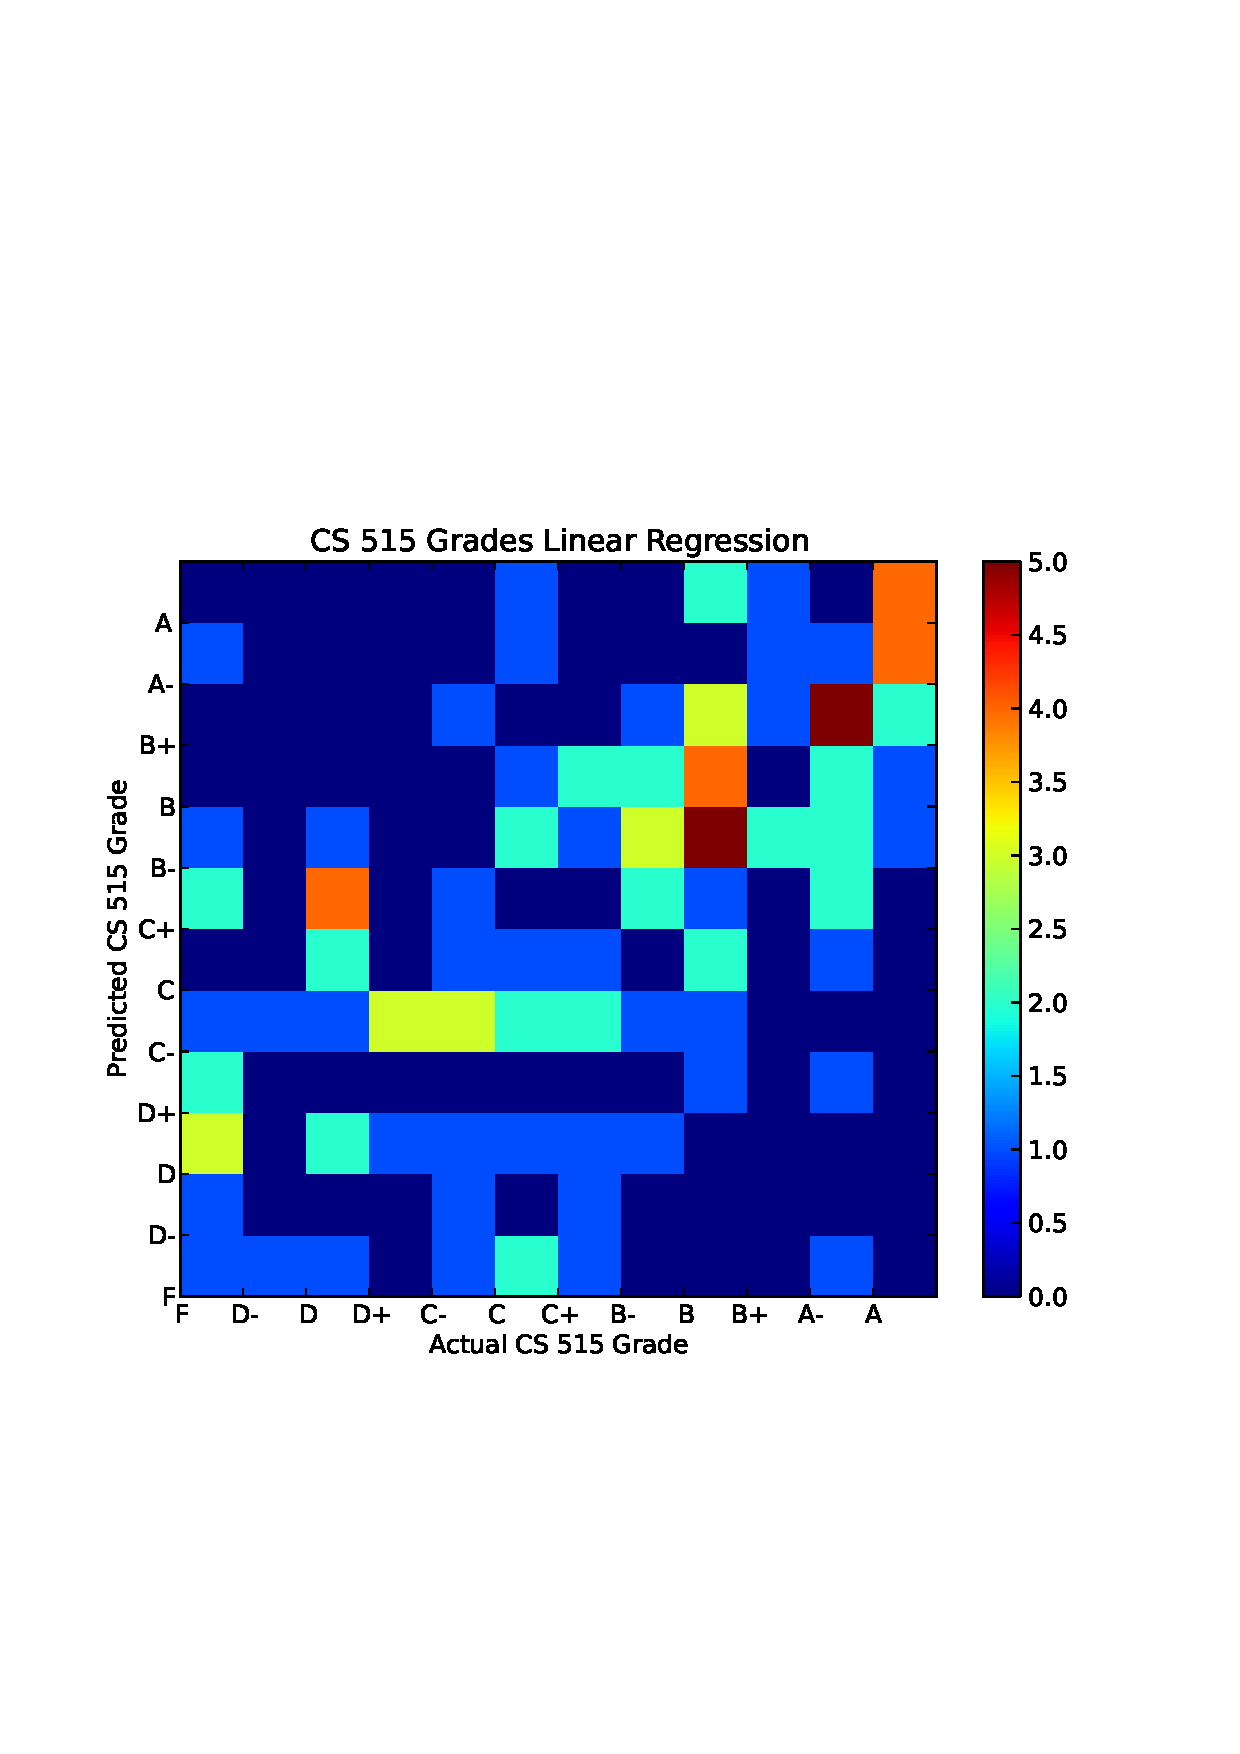
\includegraphics[width=4in]{515grade_lin.pdf}
  \caption {CS 515 Grade Linear Regression}
\label{figure:heatmaps3}
\end{figure}

\begin{figure}[h!]
\includegraphics[width=4in]{515grade_des.pdf}
  \caption {CS 515 Grade Decision Stump}
\label{figure:heatmaps4}
\end{figure}

\begin{figure}[h!]
\includegraphics[width=4in]{520grade_lin.pdf}
  \caption {CS 520 Grade Linear Regression}
\label{figure:heatmaps5}
\end{figure}

\begin{figure}[h!]
\includegraphics[width=4in]{520grade_des.pdf}
  \caption {CS 520 Grade Decision Stump}
\label{figure:heatmaps6}
\end{figure}

\begin{table}[h!]
\begin{center}
  \begin{tabular}{ r | l }
      Letter grade & Grade point \\ \hline
    A & 4.0 \\
    A- & 3.67 \\ 
    B+ & 3.33  \\ 
    B & 3.0  \\
    B- & 2.67  \\
    C+ & 2.33  \\ 
    C & 2.0  \\ 
    C- & 1.67  \\ 
    D+ & 1.33  \\ 
    D & 1.0  \\ 
    D- & 0.67  \\ 
    F, AF, WF, IC & 0 \\
      \end{tabular}
    \end{center}
  \caption {UNH Grading Scale}
\label{table:unhscale}
\end{table}

\begin{table}[h!]
\begin{center}

  \begin{tabular}{r|c|c|c|c|c|c|}
          & \multicolumn{2}{|c|}{CS 416 Grade}& \multicolumn{2}{|c|}{CS 515 Grade}& \multicolumn{2}{|c|}{CS 520 Grade} \\ \hline
                              & Lin     & Dec Stump& Lin     & Dec Stump & Lin        & Dec Stump\\ \hline
Correlation coefficient       & 0.6022  & 0.6611   & 0.5489  & 0.6211    & 0.0337     & -0.0222  \\
Mean absolute error           & 0.2014  & 0.2006   & 0.2088  & 0.1941    & 0.2569     & 0.2295   \\
Root mean squared error       & 0.3072  & 0.2551   & 0.2753  & 0.2373    & 0.3648     & 0.2955   \\
Relative absolute error       & 69.63\% & 69.32\%  & 81.65\% & 75.91\%   & 116.17\%   & 103.78\%  \\
Root relative squared error   & 90.05\% & 74.77\%  & 90.22\% & 77.76\%   & 134.46\%   & 108.92\% \\
Number samples                & 157     & 157      & 119     & 119       & 67         & 67       \\
  \end{tabular}
\end{center}
  \caption {Linear Regression vs Decision Stump Performance}
\label{table:linperform}
\end{table}


\begin{table}[h!]
\begin{center}
  \begin{tabular}{ r | l }
Weight Absolute Value & Feature   \\ \hline
2.1632 & 415 Final Grade \\
1.1064 & L \% Zeros  \\
1.0947 & R Avg  \\
0.82 & R \% Zeros  \\
0.7685 & P Max  \\
0.7363 & P Avg  \\
0.4163 & Math Class = None \\
0.4028 & OLE Avg  \\
0.3949 & Q \% Zeros  \\
0.3621 & OLE Max  \\
0.3275 & Q Avg  \\
0.3017 & Female = false \\
0.2478 & ECE major = false \\
0.2399 & L \% below 70\%  \\
0.2376 & P Diff  \\
0.1942 & P \% below 70\%  \\
0.1487 & Freshman = true \\
0.1275 & CS Major = true \\
0.104 & L Min  \\
0.0823 & Semester = 2007 \\
  \end{tabular}
\end{center}
  \caption {CS 416 Grade Weights}
\label{table:416weights}
\end{table}

\begin{table}[h!]
\begin{center}
  \begin{tabular}{ r | l }
Weight Absolute Value & Feature   \\ \hline
2.0785 & P Avg  \\
1.934 & R Avg  \\
1.6436 & P \% Zeros  \\
1.5675 & R \% Zeros  \\
0.8298 & L \% Zeros  \\
0.7348 & Q Avg  \\
0.6143 & OLE Avg  \\
0.4984 & OLE Max  \\
0.4803 & P \% below 70\%  \\
0.458 & PRE Avg  \\
0.4441 & Q \% Zeros  \\
0.325 & R Diff  \\
0.3192 & ECE major= false  \\
0.2954 & PRE \% below 70\%  \\
0.2181 & OLE Min  \\
0.2037 & Freshman = true  \\
0.2006 & P Min  \\
0.1991 & Sex unknown = false  \\
0.1915 & Math Class = Unknown  \\
0.1141 & R Min
  \end{tabular}
\end{center}
  \caption {CS 515 Grade Weights}
\label{table:515weights}
\end{table}

\begin{table}[h!]
\begin{center}
  \begin{tabular}{ r | l }
Weight Absolute Value & Feature   \\ \hline
1.0649 & R \% below 70\%  \\
1.0394 & R \% Zeros  \\
0.9173 & 415 Final Grade  \\
0.6058 & Q \% below 70\%  \\
0.4491 & OLE Min  \\
0.4422 & OLE Max  \\
0.2245 & Semester 2008 = false 
  \end{tabular}
\end{center}
  \caption {CS 520 Grade Weights}
\label{table:520weights}
\end{table}

\begin{table}[h!]
\begin{center}
\tiny
  \begin{tabular}{r|c|c|c|c|c|c|c|c|}
          & \multicolumn{2}{|c|}{Take CS 416}& \multicolumn{2}{|c|}{Take CS 515}& \multicolumn{2}{|c|}{Take CS 520}& \multicolumn{2}{|c|}{Graduate in Major} \\ \hline
                              & Log     & OneR    & Log     & OneR      & Log        & OneR     & Log        & OneR\\ \hline
Accuracy                      & 74.43\% & 70.81\% & 71.97\% & 66.24\%   & 61.34\%    & 61.34\%  & 68.57\%    & 78.57\% \\
Kappa statistic               & 0.5047  & 0.4152  & 0.2850  & 0.0158    & 0.2146     & 0.2146   & 0.2127     & 0.1491 \\
Mean absolute error           & 0.2787  & 0.2919  & 0.3015  & 0.3376    & 0.3870     & 0.3866   & 0.2097     & 0.1429 \\
Root mean squared error       & 0.4174  & 0.5403  & 0.5167  & 0.5810    & 0.6183     & 0.6217   & 0.4549     & 0.3780 \\
Relative absolute error       & 56.06\% & 58.71\% & 75.08\% & 84.07\%   & 78.34\%    & 78.24\%  & 84.88\%    & 57.82\% \\
Root relative squared error   & 83.60\% & 108.21\%& 115.14\%& 129.465\% & 123.8986\% & 124.60\% & 130.77\%   & 108.65\% \\
Number samples                & 346     & 346     & 157     & 157       & 119        & 119      & 70         & 70 \\
  \end{tabular}
\end{center}
  \caption {Logistic Regression vs OneR Performance}
\label{table:logperform}
\end{table}

\begin{table}[h!]
\begin{center}
  \begin{tabular}{ c | c | l }
Predicted YES & Predicted NO & \\ \hline
115  & 42   & Actual YES \\
43   & 146  & Actual NO \\
  \end{tabular}
\end{center}
  \caption {Take CS 416 Confusion Matrix (75.43\% correctly identified)}
\label{table:416confusion}
\end{table}

\begin{table}[h!]
\begin{center}
  \begin{tabular}{ c | c | l }
Predicted YES & Predicted NO & \\ \hline
93  & 31   & Actual YES \\
23  & 20  & Actual NO \\
  \end{tabular}
\end{center}
  \caption {Take CS 515 Confusion Matrix (71.97\% correctly identified)}
\label{table:515confusion}
\end{table}

\begin{table}[h!]
\begin{center}
  \begin{tabular}{ c | c | l }
Predicted YES & Predicted NO & \\ \hline
29   & 22   & Actual YES \\
24   & 44   & Actual NO \\
  \end{tabular}
\end{center}
  \caption {Take CS 520 Confusion Matrix (61.34\% correctly identified)}
\label{table:520confusion}
\end{table}

\begin{table}[h!]
\begin{center}
  \begin{tabular}{ c | c | l }
Predicted YES & Predicted NO & \\ \hline
8  & 8   & Actual YES \\
14   & 40  & Actual NO \\
  \end{tabular}
\end{center}
  \caption {Take CS 416 Confusion Matrix (68.57\% correctly identified)}
\label{table:gradcsconfusion}
\end{table}

\section{References}

\bibliographystyle{plain}
\bibliography{mybib.bib}

\end{document}
